\documentclass[12pt]{article}

\usepackage{titlesec}
\usepackage{geometry}
\usepackage{setspace}
\usepackage{amsmath}
\usepackage{tikz}
\usepackage{array}
\usepackage{hyperref}
\usepackage{longtable}

\geometry{margin=1in}
\setstretch{1.2}

\title{\textbf{Logical Compiler – Chart Paper Documentation}}
\author{}
\date{}

\begin{document}

\maketitle
\tableofcontents
\newpage

% -------------------------------------------------------
% ------------------ CHART 1 ----------------------------
% -------------------------------------------------------
\section{Chart 1: Lexical Analysis}

\subsection{Role of Lexical Analyzer}

\begin{center}
Source Code $\rightarrow$ Lexical Analyzer $\rightarrow$ Tokens $\rightarrow$ Parser
\end{center}

\subsection{Token Classes}

\begin{itemize}
    \item \textbf{KEYWORD} - Reserved words (CIRCUIT, INPUT, OUTPUT, WIRE, AND, OR, XOR, NAND, NOR, NOT)
    \item \textbf{IDENTIFIER} - Variable names (A, B, Sum, Carry, etc.)
    \item \textbf{LBRACE} - Left brace \{
    \item \textbf{RBRACE} - Right brace \}
    \item \textbf{LPAREN} - Left parenthesis (
    \item \textbf{RPAREN} - Right parenthesis )
    \item \textbf{SEMICOLON} - Semicolon ;
    \item \textbf{COMMA} - Comma ,
    \item \textbf{EQUALS} - Equals sign =
\end{itemize}

\subsection{Token Specifications (Regex)}

\begin{verbatim}
KEYWORD      → \b(CIRCUIT|INPUT|OUTPUT|WIRE|AND|OR|XOR|NAND|NOR|NOT)\b
IDENTIFIER   → [a-zA-Z_][a-zA-Z0-9_]*
LBRACE       → \{
RBRACE       → \}
LPAREN       → \(
RPAREN       → \)
SEMICOLON    → ;
COMMA        → ,
EQUALS       → =
WHITESPACE   → [ \t]+
NEWLINE      → \n
\end{verbatim}

\subsection{DFA Transition Table}

\begin{center}
\begin{tabular}{|c|c|c|c|}
\hline
\textbf{Char Class} & \textbf{q0} & \textbf{q1} & \textbf{q2} \\
\hline
letter (a-z, A-Z) & q1 & q1 & - \\
underscore (\_) & q1 & q1 & - \\
digit (0-9) & q2 & q1 & q2 \\
other & q2 & q2 & q2 \\
\hline
\end{tabular}
\end{center}

\textbf{States:}
\begin{itemize}
    \item \textbf{q0}: Start state (initial)
    \item \textbf{q1}: Accepting state (valid identifier) - double circle
    \item \textbf{q2}: Dead state (reject)
\end{itemize}

\subsection{Dry Run Example: Half Adder Input}

\textbf{Input Source Code:}
\begin{verbatim}
CIRCUIT HalfAdder {
  INPUT A, B;
  OUTPUT Sum, Carry;
  Sum = XOR(A, B);
  Carry = AND(A, B);
}
\end{verbatim}

\textbf{Tokenization Process:}

\begin{center}
\begin{longtable}{|c|c|c|}
\hline
\textbf{Character/Token} & \textbf{State/Token Type} & \textbf{Token Generated} \\
\hline
\endfirsthead
\hline
\textbf{Character/Token} & \textbf{State/Token Type} & \textbf{Token Generated} \\
\hline
\endhead
CIRCUIT & KEYWORD & Token(KEYWORD, 'CIRCUIT', L1:C1) \\
HalfAdder & IDENTIFIER (q0→q1→q1→...) & Token(IDENTIFIER, 'HalfAdder', L1:C9) \\
\{ & LBRACE & Token(LBRACE, '\{', L1:C20) \\
INPUT & KEYWORD & Token(KEYWORD, 'INPUT', L2:C3) \\
A & IDENTIFIER (q0→q1) & Token(IDENTIFIER, 'A', L2:C9) \\
, & COMMA & Token(COMMA, ',', L2:C10) \\
B & IDENTIFIER (q0→q1) & Token(IDENTIFIER, 'B', L2:C12) \\
; & SEMICOLON & Token(SEMICOLON, ';', L2:C13) \\
OUTPUT & KEYWORD & Token(KEYWORD, 'OUTPUT', L3:C3) \\
Sum & IDENTIFIER (q0→q1→q1→q1) & Token(IDENTIFIER, 'Sum', L3:C10) \\
, & COMMA & Token(COMMA, ',', L3:C13) \\
Carry & IDENTIFIER (q0→q1→...) & Token(IDENTIFIER, 'Carry', L3:C15) \\
; & SEMICOLON & Token(SEMICOLON, ';', L3:C20) \\
Sum & IDENTIFIER & Token(IDENTIFIER, 'Sum', L4:C3) \\
= & EQUALS & Token(EQUALS, '=', L4:C7) \\
XOR & KEYWORD & Token(KEYWORD, 'XOR', L4:C9) \\
( & LPAREN & Token(LPAREN, '(', L4:C12) \\
A & IDENTIFIER & Token(IDENTIFIER, 'A', L4:C13) \\
, & COMMA & Token(COMMA, ',', L4:C14) \\
B & IDENTIFIER & Token(IDENTIFIER, 'B', L4:C16) \\
) & RPAREN & Token(RPAREN, ')', L4:C17) \\
; & SEMICOLON & Token(SEMICOLON, ';', L4:C18) \\
Carry & IDENTIFIER & Token(IDENTIFIER, 'Carry', L5:C3) \\
= & EQUALS & Token(EQUALS, '=', L5:C9) \\
AND & KEYWORD & Token(KEYWORD, 'AND', L5:C11) \\
( & LPAREN & Token(LPAREN, '(', L5:C14) \\
A & IDENTIFIER & Token(IDENTIFIER, 'A', L5:C15) \\
, & COMMA & Token(COMMA, ',', L5:C16) \\
B & IDENTIFIER & Token(IDENTIFIER, 'B', L5:C18) \\
) & RPAREN & Token(RPAREN, ')', L5:C19) \\
; & SEMICOLON & Token(SEMICOLON, ';', L5:C20) \\
\} & RBRACE & Token(RBRACE, '\}', L6:C1) \\
\hline
\end{longtable}
\end{center}

\textbf{Total Tokens Generated:} 28 tokens

\newpage

% -------------------------------------------------------
% ------------------ CHART 2 ----------------------------
% -------------------------------------------------------
\section{Chart 2: LL(1) Parser}

\subsection{Grammar (Left Recursion Removed)}

\begin{verbatim}
<program> ::= CIRCUIT <identifier> <lbrace> <declarations> <gates> <rbrace>

<declarations> ::= <declaration> <declarations>
                 | ε

<declaration> ::= <declaration_keyword> <identifier_list> <semicolon>

<declaration_keyword> ::= INPUT | OUTPUT | WIRE

<identifier_list> ::= <identifier> <identifier_list_tail>

<identifier_list_tail> ::= <comma> <identifier> <identifier_list_tail>
                          | ε

<gates> ::= <gate> <gates>
          | ε

<gate> ::= <identifier> <equals> <gate_type> <lparen> <gate_inputs> <rparen> <semicolon>

<gate_type> ::= AND | OR | XOR | NAND | NOR | NOT

<gate_inputs> ::= <identifier> <gate_inputs_tail>

<gate_inputs_tail> ::= <comma> <identifier> <gate_inputs_tail>
                      | ε
\end{verbatim}

\subsection{FIRST and FOLLOW Sets}

\textbf{FIRST Sets:}
\begin{itemize}
    \item FIRST(program) = \{CIRCUIT\}
    \item FIRST(declarations) = \{INPUT, OUTPUT, WIRE, ε\}
    \item FIRST(declaration) = \{INPUT, OUTPUT, WIRE\}
    \item FIRST(identifier\_list) = \{IDENTIFIER\}
    \item FIRST(gates) = \{IDENTIFIER, ε\}
    \item FIRST(gate) = \{IDENTIFIER\}
    \item FIRST(gate\_type) = \{AND, OR, XOR, NAND, NOR, NOT\}
\end{itemize}

\textbf{FOLLOW Sets:}
\begin{itemize}
    \item FOLLOW(declarations) = \{IDENTIFIER, \}\}
    \item FOLLOW(gates) = \{\}\}
    \item FOLLOW(identifier\_list) = \{;\}
    \item FOLLOW(gate\_inputs) = \{)\}
\end{itemize}

\subsection{LL(1) Predictive Parsing Table}

\begin{center}
\small
\begin{tabular}{|c|c|c|c|c|c|c|c|}
\hline
\textbf{Non-Terminal} & \textbf{CIRCUIT} & \textbf{INPUT/OUTPUT/WIRE} & \textbf{IDENTIFIER} & \textbf{\{} & \textbf{\}} & \textbf{;} & \textbf{\$} \\
\hline
program & program & - & - & - & - & - & - \\
\hline
declarations & - & declaration declarations & ε & - & ε & - & - \\
\hline
gates & - & - & gate gates & - & ε & - & - \\
\hline
\end{tabular}
\end{center}

\subsection{LL(1) Parsing Example: Half Adder}

\textbf{Input:} CIRCUIT HalfAdder \{ INPUT A , B ; OUTPUT Sum , Carry ; Sum = XOR ( A , B ) ; Carry = AND ( A , B ) ; \}

\begin{center}
\begin{longtable}{|c|c|c|}
\hline
\textbf{Stack} & \textbf{Input} & \textbf{Action} \\
\hline
\endfirsthead
\hline
\textbf{Stack} & \textbf{Input} & \textbf{Action} \\
\hline
\endhead
\$ program & CIRCUIT HalfAdder \{ ... \$ & Expand E → CIRCUIT identifier \{ declarations gates \} \\
\$ \} gates declarations \{ identifier CIRCUIT & CIRCUIT HalfAdder \{ ... \$ & Match CIRCUIT \\
\$ \} gates declarations \{ identifier & HalfAdder \{ ... \$ & Match identifier \\
\$ \} gates declarations \{ & \{ ... \$ & Match \{ \\
\$ \} gates declarations & INPUT A , B ; ... \$ & Expand declarations → declaration declarations \\
\$ \} gates declarations declaration & INPUT A , B ; ... \$ & Expand declaration → INPUT identifier\_list ; \\
\$ \} gates declarations ; identifier\_list INPUT & INPUT A , B ; ... \$ & Match INPUT \\
\$ \} gates declarations ; identifier\_list & A , B ; ... \$ & Expand identifier\_list → identifier identifier\_list\_tail \\
\$ \} gates declarations ; identifier\_list\_tail identifier & A , B ; ... \$ & Match identifier (A) \\
\$ \} gates declarations ; identifier\_list\_tail & , B ; ... \$ & Expand identifier\_list\_tail → , identifier identifier\_list\_tail \\
\$ \} gates declarations ; identifier\_list\_tail identifier , & , B ; ... \$ & Match , \\
\$ \} gates declarations ; identifier\_list\_tail identifier & B ; ... \$ & Match identifier (B) \\
\$ \} gates declarations ; identifier\_list\_tail & ; ... \$ & Expand identifier\_list\_tail → ε \\
\$ \} gates declarations ; & ; ... \$ & Match ; \\
\$ \} gates declarations & OUTPUT Sum , Carry ; ... \$ & Expand declarations → declaration declarations \\
\$ \} gates & Sum = XOR ( A , B ) ; ... \$ & Expand declarations → ε \\
\$ \} gates & Sum = XOR ( A , B ) ; ... \$ & Expand gates → gate gates \\
\$ \} gates gate & Sum = XOR ( A , B ) ; ... \$ & Expand gate → identifier = gate\_type ( gate\_inputs ) ; \\
\$ \} gates ; ) gate\_inputs ( gate\_type = identifier & Sum = XOR ( A , B ) ; ... \$ & Match identifier (Sum) \\
\$ \} gates ; ) gate\_inputs ( gate\_type = & = XOR ( A , B ) ; ... \$ & Match = \\
\$ \} gates ; ) gate\_inputs ( gate\_type & XOR ( A , B ) ; ... \$ & Match gate\_type (XOR) \\
\$ \} gates ; ) gate\_inputs ( & ( A , B ) ; ... \$ & Match ( \\
\$ \} gates ; ) gate\_inputs & A , B ) ; ... \$ & Expand gate\_inputs → identifier gate\_inputs\_tail \\
\$ \} gates ; ) gate\_inputs\_tail identifier & A , B ) ; ... \$ & Match identifier (A) \\
\$ \} gates ; ) gate\_inputs\_tail & , B ) ; ... \$ & Expand gate\_inputs\_tail → , identifier gate\_inputs\_tail \\
\$ \} gates ; ) gate\_inputs\_tail identifier , & , B ) ; ... \$ & Match , \\
\$ \} gates ; ) gate\_inputs\_tail identifier & B ) ; ... \$ & Match identifier (B) \\
\$ \} gates ; ) gate\_inputs\_tail & ) ; ... \$ & Expand gate\_inputs\_tail → ε \\
\$ \} gates ; ) & ) ; ... \$ & Match ) \\
\$ \} gates ; & ; ... \$ & Match ; \\
\$ \} gates & Carry = AND ( A , B ) ; ... \$ & Expand gates → gate gates \\
\$ \} gates gate & Carry = AND ( A , B ) ; ... \$ & Expand gate → identifier = gate\_type ( gate\_inputs ) ; \\
\$ \} gates & \} ... \$ & Expand gates → ε \\
\$ \} & \} ... \$ & Match \} \\
\$ & \$ & ACCEPT \\
\hline
\end{longtable}
\end{center}

\newpage

% -------------------------------------------------------
% ------------------ CHART 3 ----------------------------
% -------------------------------------------------------
\section{Chart 3: LR(0) Parser}

\subsection{Augmented Grammar}

\begin{verbatim}
(0) S' → program
(1) program → CIRCUIT identifier { declarations gates }
(2) declarations → declaration declarations
(3) declarations → ε
(4) declaration → INPUT identifier_list ;
(5) declaration → OUTPUT identifier_list ;
(6) declaration → WIRE identifier_list ;
(7) identifier_list → identifier identifier_list_tail
(8) identifier_list_tail → , identifier identifier_list_tail
(9) identifier_list_tail → ε
(10) gates → gate gates
(11) gates → ε
(12) gate → identifier = gate_type ( gate_inputs ) ;
(13) gate_inputs → identifier gate_inputs_tail
(14) gate_inputs_tail → , identifier gate_inputs_tail
(15) gate_inputs_tail → ε
\end{verbatim}

\subsection{LR(0) Items}

\textbf{State I0:}
\begin{verbatim}
S' → .program
program → .CIRCUIT identifier { declarations gates }
\end{verbatim}

\textbf{State I1:}
\begin{verbatim}
S' → program.
\end{verbatim}

\textbf{State I2:}
\begin{verbatim}
program → CIRCUIT .identifier { declarations gates }
\end{verbatim}

\textbf{State I3:}
\begin{verbatim}
program → CIRCUIT identifier .{ declarations gates }
\end{verbatim}

\textbf{State I4:}
\begin{verbatim}
program → CIRCUIT identifier { .declarations gates }
declarations → .declaration declarations
declarations → .ε
declaration → .INPUT identifier_list ;
declaration → .OUTPUT identifier_list ;
declaration → .WIRE identifier_list ;
\end{verbatim}

\subsection{LR(0) Automaton}

(Draw states I0, I1, I2, I3, I4, ... using tikz or by hand on chart)

\textbf{Key States:}
\begin{itemize}
    \item I0: Initial state (start)
    \item I1: Accept state (S' → program.)
    \item I2-I4: Processing program structure
    \item I5+: Processing declarations and gates
\end{itemize}

\subsection{LR(0) Parsing Table}

\begin{center}
\small
\begin{tabular}{|c|c|c|c|c|c|c|c|c|}
\hline
\textbf{State} & \textbf{CIRCUIT} & \textbf{identifier} & \textbf{\{} & \textbf{INPUT} & \textbf{OUTPUT} & \textbf{;} & \textbf{\}} & \textbf{ACTION} \\
\hline
I0 & S2 & - & - & - & - & - & - & - \\
I1 & - & - & - & - & - & - & - & ACCEPT \\
I2 & - & S3 & - & - & - & - & - & - \\
I3 & - & - & S4 & - & - & - & - & - \\
I4 & - & - & - & S5 & S6 & - & R3 & - \\
\hline
\end{tabular}
\end{center}

\subsection{Shift–Reduce Dry Run: Half Adder}

\textbf{Input:} CIRCUIT HalfAdder \{ INPUT A , B ; OUTPUT Sum , Carry ; Sum = XOR ( A , B ) ; Carry = AND ( A , B ) ; \}

\begin{center}
\begin{longtable}{|c|c|c|c|}
\hline
\textbf{Stack} & \textbf{Input} & \textbf{Action} \\
\hline
\endfirsthead
\hline
\textbf{Stack} & \textbf{Input} & \textbf{Action} \\
\hline
\endhead
0 & CIRCUIT HalfAdder \{ ... \$ & SHIFT (goto I2) \\
0 CIRCUIT 2 & HalfAdder \{ ... \$ & SHIFT identifier (goto I3) \\
0 CIRCUIT 2 identifier 3 & \{ ... \$ & SHIFT \{ (goto I4) \\
0 CIRCUIT 2 identifier 3 \{ 4 & INPUT A , B ; ... \$ & SHIFT INPUT (goto I5) \\
0 ... 4 INPUT 5 & A , B ; ... \$ & SHIFT identifier \\
0 ... 5 identifier & , B ; ... \$ & SHIFT , \\
0 ... 5 identifier , & B ; ... \$ & SHIFT identifier \\
0 ... 5 identifier , identifier & ; ... \$ & REDUCE identifier\_list\_tail → ε \\
0 ... 5 identifier\_list & ; ... \$ & SHIFT ; \\
0 ... 5 identifier\_list ; & ... \$ & REDUCE declaration → INPUT identifier\_list ; \\
0 ... 4 declaration & OUTPUT Sum , Carry ; ... \$ & REDUCE declarations → declaration declarations \\
0 ... 4 declarations & OUTPUT Sum , Carry ; ... \$ & SHIFT OUTPUT \\
... & ... & ... \\
0 ... & \} ... \$ & REDUCE gates → ε \\
0 ... declarations gates & \} ... \$ & SHIFT \} \\
0 ... & \$ & REDUCE program → ... \\
0 program & \$ & ACCEPT \\
\hline
\end{longtable}
\end{center}

\newpage

% -------------------------------------------------------
% ------------------ CHART 4 ----------------------------
% -------------------------------------------------------
\section{Chart 4: SLR(1) Parser}

\subsection{FOLLOW Sets}

\textbf{FOLLOW Sets (Required for SLR reduce actions):}
\begin{itemize}
    \item FOLLOW(program) = \{\$\}
    \item FOLLOW(declarations) = \{IDENTIFIER, \}\}
    \item FOLLOW(declaration) = \{INPUT, OUTPUT, WIRE, IDENTIFIER, \}\}
    \item FOLLOW(identifier\_list) = \{;\}
    \item FOLLOW(identifier\_list\_tail) = \{;\}
    \item FOLLOW(gates) = \{\}\}
    \item FOLLOW(gate) = \{IDENTIFIER, \}\}
    \item FOLLOW(gate\_inputs) = \{)\}
    \item FOLLOW(gate\_inputs\_tail) = \{)\}
\end{itemize}

\subsection{SLR Table Construction}

Use FOLLOW sets + LR(0) items to resolve reduce actions.

\textbf{Key Rule:} Reduce by production A → α only when lookahead ∈ FOLLOW(A)

\subsection{Typical Conflict Resolution}

\textbf{Shift/Reduce Conflict Resolution:}
\begin{itemize}
    \item If lookahead ∈ FOLLOW(A), use REDUCE
    \item Otherwise, use SHIFT
    \item Example: In state with item "declarations → declaration declarations."
        \begin{itemize}
            \item If lookahead = IDENTIFIER or \}, REDUCE by declarations → declaration declarations
            \item Otherwise, SHIFT
        \end{itemize}
\end{itemize}

\subsection{SLR Parsing Example: Half Adder}

\textbf{SLR Parsing Table (Partial):}

\begin{center}
\small
\begin{tabular}{|c|c|c|c|c|c|c|c|}
\hline
\textbf{State} & \textbf{INPUT} & \textbf{OUTPUT} & \textbf{identifier} & \textbf{;} & \textbf{\}} & \textbf{\$} & \textbf{ACTION} \\
\hline
I4 & S5 & S6 & - & - & R3 & - & declarations → ε \\
I5 & - & - & S7 & - & - & - & - \\
I6 & - & - & S7 & - & - & - & - \\
I7 & - & - & S8 & R9 & - & - & identifier\_list\_tail → ε \\
I8 & - & - & - & R8 & - & - & identifier\_list\_tail → , identifier ... \\
\hline
\end{tabular}
\end{center}

\textbf{Parsing Moves:}
\begin{verbatim}
Stack: 0 CIRCUIT 2 identifier 3 { 4
Input: INPUT A , B ; OUTPUT ...
Action: SHIFT INPUT (goto I5)

Stack: ... 4 INPUT 5
Input: A , B ; OUTPUT ...
Action: SHIFT identifier (goto I7)

Stack: ... 5 identifier 7
Input: , B ; OUTPUT ...
Action: SHIFT , (goto I8)

Stack: ... 7 , 8
Input: B ; OUTPUT ...
Action: SHIFT identifier (goto I7)

Stack: ... 8 identifier 7
Input: ; OUTPUT ...
Action: REDUCE identifier_list_tail → ε (lookahead ; ∈ FOLLOW)
Action: REDUCE identifier_list → identifier identifier_list_tail
Action: SHIFT ; (goto I9)
Action: REDUCE declaration → INPUT identifier_list ;
\end{verbatim}

\newpage

% -------------------------------------------------------
% ------------------ CHART 5 ----------------------------
% -------------------------------------------------------
\section{Chart 5: LALR(1) Parser}

\subsection{LR(1) Items Example}

\textbf{LR(1) Item Format:} [A → α . β, lookahead]

\textbf{Example Items:}
\begin{verbatim}
[declarations → declaration .declarations, {IDENTIFIER, } }]
[declarations → declaration .declarations, {$}]
[gates → gate .gates, {}}]
[gates → gate .gates, {$}]
\end{verbatim}

\subsection{Merging LR(1) Item Sets}

\textbf{Illustration:}

\textbf{State I10 (LR(1)):}
\begin{verbatim}
[declarations → declaration .declarations, {IDENTIFIER}]
[declarations → declaration .declarations, {}}]
\end{verbatim}

\textbf{State I11 (LR(1)):}
\begin{verbatim}
[declarations → declaration .declarations, {$}]
\end{verbatim}

\textbf{Merged LALR State I10':}
\begin{verbatim}
[declarations → declaration .declarations, {IDENTIFIER, }, $}]
\end{verbatim}

\textbf{Key Points:}
\begin{itemize}
    \item Two states with same core (declarations → declaration .declarations)
    \item Merge lookaheads: {IDENTIFIER, }, $} ∪ {$} = {IDENTIFIER, }, $}
    \item Result: Single LALR state with merged lookaheads
\end{itemize}

\subsection{LALR Table}

\textbf{ACTION/GOTO Table (Partial):}

\begin{center}
\small
\begin{tabular}{|c|c|c|c|c|c|}
\hline
\textbf{State} & \textbf{IDENTIFIER} & \textbf{;} & \textbf{\}} & \textbf{\$} & \textbf{GOTO} \\
\hline
I10' & S/R & - & R & R & declarations \\
I12' & S & R & R & R & gates \\
\hline
\end{tabular}
\end{center}

\subsection{Why LALR is Used in Compilers}

\begin{itemize}
    \item \textbf{Compact tables:} Fewer states than CLR(1)
    \item \textbf{Same power as LR(1):} Handles most practical grammars
    \item \textbf{Efficient:} Faster table construction than CLR(1)
    \item \textbf{Widely used:} Yacc/Bison use LALR(1)
\end{itemize}

\newpage

% -------------------------------------------------------
% ------------------ CHART 6 ----------------------------
% -------------------------------------------------------
\section{Chart 6: Canonical LR(1) (CLR) Parser}

\subsection{LR(1) Items}

\textbf{General form:} [A → α . β, lookahead]

Where:
\begin{itemize}
    \item A → α β is a production
    \item The dot (.) marks the current position
    \item lookahead is a set of terminal symbols
\end{itemize}

\textbf{Example LR(1) Items:}
\begin{verbatim}
[program → CIRCUIT identifier { .declarations gates }, {$}]
[declarations → .declaration declarations, {IDENTIFIER}]
[declarations → .declaration declarations, {}}]
[declarations → .ε, {IDENTIFIER}]
[declarations → .ε, {}}]
[gate → identifier = gate_type ( .gate_inputs ) ;, {IDENTIFIER}]
[gate → identifier = gate_type ( .gate_inputs ) ;, {}}]
\end{verbatim}

\subsection{Closure and GOTO Examples}

\textbf{Closure Operation:}
\begin{verbatim}
CLOSURE(I) = I ∪ {[B → .γ, b] | [A → α .Bβ, a] ∈ I, 
                   B → γ is production, b ∈ FIRST(βa)}
\end{verbatim}

\textbf{Example:}
\begin{verbatim}
I = {[declarations → .declaration declarations, {IDENTIFIER}]}

CLOSURE(I) adds:
[declaration → .INPUT identifier_list ;, {IDENTIFIER}]
[declaration → .OUTPUT identifier_list ;, {IDENTIFIER}]
[declaration → .WIRE identifier_list ;, {IDENTIFIER}]
\end{verbatim}

\textbf{GOTO Operation:}
\begin{verbatim}
GOTO(I, X) = CLOSURE({[A → αX .β, a] | [A → α .Xβ, a] ∈ I})
\end{verbatim}

\subsection{CLR Automaton (Partial)}

\textbf{State I0:}
\begin{verbatim}
[S' → .program, {$}]
[program → .CIRCUIT identifier { declarations gates }, {$}]
\end{verbatim}

\textbf{State I1:}
\begin{verbatim}
[S' → program., {$}]
\end{verbatim}

\textbf{State I4a:}
\begin{verbatim}
[declarations → .declaration declarations, {IDENTIFIER}]
[declarations → .ε, {IDENTIFIER}]
[declaration → .INPUT identifier_list ;, {IDENTIFIER}]
[declaration → .OUTPUT identifier_list ;, {IDENTIFIER}]
\end{verbatim}

\textbf{State I4b:}
\begin{verbatim}
[declarations → .declaration declarations, {}}]
[declarations → .ε, {}}]
[declaration → .INPUT identifier_list ;, {}}]
[declaration → .OUTPUT identifier_list ;, {}}]
\end{verbatim}

\textbf{Note:} I4a and I4b have same core but different lookaheads (not merged in CLR)

\subsection{CLR Parsing Table}

\textbf{Difference from LALR:}
\begin{itemize}
    \item \textbf{CLR:} Separate states for different lookaheads (more states)
    \item \textbf{LALR:} Merged states with combined lookaheads (fewer states)
    \item \textbf{Example:} CLR has I4a and I4b separately; LALR merges them into I4'
\end{itemize}

\textbf{CLR Table (Partial):}
\begin{center}
\small
\begin{tabular}{|c|c|c|c|c|}
\hline
\textbf{State} & \textbf{INPUT} & \textbf{IDENTIFIER} & \textbf{\}} & \textbf{\$} \\
\hline
I4a & S5 & R3 & - & - \\
I4b & S5 & - & R3 & - \\
\hline
\end{tabular}
\end{center}

\newpage

% -------------------------------------------------------
% ------------------ CHART 7 ----------------------------
% -------------------------------------------------------
\section{Chart 7: Semantic Analysis}

\subsection{Role of Semantic Analysis}

\begin{itemize}
    \item Type checking (validate gate input counts)
    \item Scope management (symbol table construction)
    \item Semantic error detection (undeclared identifiers, cycles)
    \item Output assignment verification
\end{itemize}

\subsection{Annotated Parse Tree}

\textbf{Half Adder Parse Tree:}
\begin{verbatim}
Program(HalfAdder) [symbol_table: {A, B, Sum, Carry}]
├── Declaration(INPUT, [A, B]) [adds A, B to symbol_table]
│   ├── identifier_list [A, B]
│   └── semicolon
├── Declaration(OUTPUT, [Sum, Carry]) [adds Sum, Carry to symbol_table]
│   ├── identifier_list [Sum, Carry]
│   └── semicolon
├── Gate(Sum = XOR(A, B)) [checks: A∈symbol_table, B∈symbol_table, 
│   │                        XOR has 2 inputs ✓, assigns Sum]
│   ├── identifier (Sum)
│   ├── equals (=)
│   ├── gate_type (XOR)
│   ├── gate_inputs [A, B]
│   └── semicolon
└── Gate(Carry = AND(A, B)) [checks: A∈symbol_table, B∈symbol_table,
                              AND has 2 inputs ✓, assigns Carry]
    ├── identifier (Carry)
    ├── equals (=)
    ├── gate_type (AND)
    ├── gate_inputs [A, B]
    └── semicolon
\end{verbatim}

\subsection{Symbol Table Example: Half Adder}

\begin{center}
\begin{tabular}{|c|c|c|c|c|}
\hline
\textbf{Name} & \textbf{Category} & \textbf{Defined} & \textbf{Source Gate} & \textbf{Used By} \\
\hline
A & INPUT & Yes & - & Sum, Carry \\
B & INPUT & Yes & - & Sum, Carry \\
Sum & OUTPUT & Yes & Gate(Sum = XOR(A, B)) & - \\
Carry & OUTPUT & Yes & Gate(Carry = AND(A, B)) & - \\
\hline
\end{tabular}
\end{center}

\subsection{Semantic Rules}

\textbf{Rule 1: Declaration Check}
\begin{verbatim}
Gate → identifier = gate_type ( gate_inputs ) ;

For each input_id in gate_inputs:
    if input_id ∉ symbol_table:
        ERROR: Undeclared identifier
\end{verbatim}

\textbf{Rule 2: Gate Input Count Validation}
\begin{verbatim}
if gate_type == NOT and len(gate_inputs) != 1:
    ERROR: NOT requires 1 input
if gate_type in {AND, OR, XOR, NAND, NOR} and len(gate_inputs) != 2:
    ERROR: Gate requires 2 inputs
\end{verbatim}

\textbf{Rule 3: Output Assignment}
\begin{verbatim}
For each OUTPUT identifier:
    if identifier not assigned by any gate:
        ERROR: OUTPUT never assigned
\end{verbatim}

\textbf{Rule 4: Input Assignment Prevention}
\begin{verbatim}
For gate with output identifier:
    if identifier.category == INPUT:
        ERROR: Cannot assign to INPUT
\end{verbatim}

\textbf{Rule 5: Cycle Detection}
\begin{verbatim}
Use DFS to detect cycles:
    if cycle found in dependency graph:
        ERROR: Combinational cycle detected
\end{verbatim}

\subsection{Semantic Analysis Result: Half Adder}

\textbf{Status:} ✓ PASSED

\textbf{Checks Performed:}
\begin{itemize}
    \item ✓ All identifiers declared (A, B, Sum, Carry)
    \item ✓ Gate input counts valid (XOR: 2 inputs, AND: 2 inputs)
    \item ✓ All OUTPUTs assigned (Sum, Carry)
    \item ✓ No INPUT assignments
    \item ✓ No cycles detected
\end{itemize}

\textbf{Symbol Table Entries:} 4

\textbf{Errors:} None

\newpage

% -------------------------------------------------------
% ------------------ CHART 8 ----------------------------
% -------------------------------------------------------
\section{Chart 8: Intermediate Code Generation + Optimization}

\subsection{Three-Address Code}

\textbf{Format:} (Operation, Argument1, Argument2, Result)

\textbf{Half Adder Example:}
\begin{verbatim}
(1) Sum = XOR(A, B)
(2) Carry = AND(A, B)
\end{verbatim}

\textbf{Quadruple Representation:}
\begin{center}
\begin{tabular}{|c|c|c|c|c|}
\hline
\textbf{No.} & \textbf{Operation} & \textbf{Arg1} & \textbf{Arg2} & \textbf{Result} \\
\hline
1 & XOR & A & B & Sum \\
2 & AND & A & B & Carry \\
\hline
\end{tabular}
\end{center}

\subsection{Basic Blocks and Flow}

\textbf{Control Flow Graph (CFG) for Half Adder:}

\begin{center}
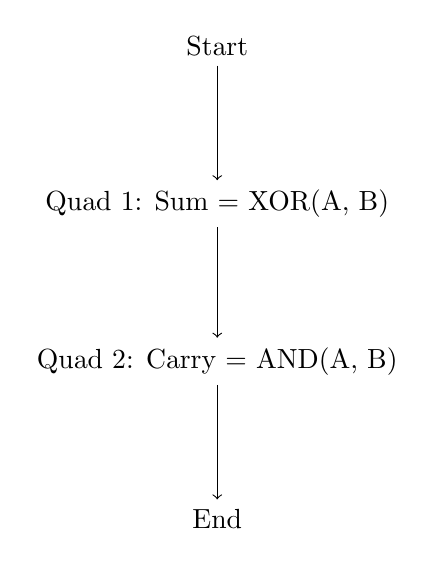
\begin{tikzpicture}[node distance=2cm, auto]
    \node (start) {Start};
    \node [below of=start] (q1) {Quad 1: Sum = XOR(A, B)};
    \node [below of=q1] (q2) {Quad 2: Carry = AND(A, B)};
    \node [below of=q2] (end) {End};
    
    \draw[->] (start) -- (q1);
    \draw[->] (q1) -- (q2);
    \draw[->] (q2) -- (end);
\end{tikzpicture}
\end{center}

\textbf{Basic Block:} Single block with sequential execution (no branches)

\subsection{Optimizations}

\textbf{1. Constant Folding}
\begin{verbatim}
AND(A, 0) → 0
AND(A, 1) → A
OR(A, 1) → 1
OR(A, 0) → A
XOR(A, 0) → A
XOR(A, A) → 0
\end{verbatim}

\textbf{2. Dead Code Elimination}
\begin{verbatim}
Remove computations whose results are never used.
Example: temp = AND(A, 0); (if temp never used)
\end{verbatim}

\textbf{3. Copy Propagation}
\begin{verbatim}
Replace uses of a variable with its assigned value.
Example: temp = A; Sum = XOR(temp, B) → Sum = XOR(A, B)
\end{verbatim}

\textbf{4. Common Subexpression Elimination}
\begin{verbatim}
Identify and reuse common computations.
Example: If both gates use XOR(A, B), compute once and reuse.
\end{verbatim}

\subsection{Optimization Process: Half Adder}

\textbf{Before Optimization:}
\begin{verbatim}
(1) Sum = XOR(A, B)
(2) Carry = AND(A, B)
\end{verbatim}

\textbf{Optimization Analysis:}
\begin{itemize}
    \item No constants to fold
    \item No dead code (both outputs used)
    \item No copy propagation needed
    \item No common subexpressions (different operations)
\end{itemize}

\textbf{After Optimization:}
\begin{verbatim}
(1) Sum = XOR(A, B)
(2) Carry = AND(A, B)
\end{verbatim}

\textbf{Result:} No changes (already optimal)

\subsection{Final Machine-like Code (Python)}

\textbf{Generated Code:}
\begin{verbatim}
def simulate(A, B):
    Sum = A ^ B      # XOR operation
    Carry = A & B    # AND operation
    return Sum, Carry
\end{verbatim}

\textbf{Execution:}
\begin{verbatim}
A  B || Sum  Carry
0  0 || 0    0
0  1 || 1    0
1  0 || 1    0
1  1 || 0    1
\end{verbatim}

\end{document}
